\documentclass[a4paper, 12pt]{article}

\usepackage{wrapfig}
\usepackage{graphicx}
\usepackage{mathtext}
\usepackage{amsmath}
\usepackage{siunitx} % Required for alignment
\usepackage{multirow}
\usepackage{gensymb}
\usepackage{rotating}
\sisetup{
  round-mode          = places, % Rounds numbers
  round-precision     = 2, % to 2 places
}

\usepackage[T1,T2A]{fontenc}

\usepackage[russian]{babel}

\graphicspath{{pictures/}}


\title{\begin{center}Лабораторная работа №1.2.5\end{center}
Иследование прецессии уравновешенного гироскопа}
\author{Мыздриков И.В., Б06-401}
\date{\today}

\begin{document}
    \pagenumbering{gobble}
    \maketitle
    \newpage
    \pagenumbering{arabic}

    \section{Ход работы}
    \paragraph{}
    Сначала установим параметры системы.
    \begin{align*}
     l&=(120\pm1)мм\\
     g&=(9.8155\pm0.0005)мс^{-2}\\
    \end{align*}

    \paragraph{}
    Приведем данные, полученные при измерениях.

    \begin{table}[h!]
        \begin{center}
        \begin{tabular}{|l|r|r|r|r|r|}
        \hline
        $№$ & $m, г$ &   $N$ & $t, с$ & $T, с$\\\hline
        1  &  335,5 &  5 &  151 & 30.2 \\
        2  &  296,0 &  5 &  188 & 37,6 \\
        3  &  213,3 &  5 &  238 & 47,6 \\
        4  &  173,7 &  5 &  292 & 58,4 \\
        5  &  138,0 &  5 &  368 & 73,6 \\
      
        \hline
        \end{tabular}
         \caption{Измерения периода прецессии при различных массах груза}
        \end{center}

    \end{table}

    \paragraph{}
    Отсюда обработав данные получаем следующие значения


    \begin{table}[h!]
        \begin{center}
        \begin{tabular}{|l|r|r|r|}
        \hline
        $№$ & $m, г$ &   $T, с$ & $\Omega, с^{-1}$ \\\hline
        1 &  335,5 &  30,2 &   0.208 \\
        2 &  296,0 &  37,6 &   0.167 \\
        3 &  213,3 &  47,6 &   0.1320 \\
        4 &  173,7 &  58,4 &   0.1076  \\
        5 &  138,0 &  30.4 &   0.0854  \\
        \hline
        \end{tabular}
         \caption{Обработанные данные}
        \end{center}

    \end{table}
    \paragraph{}
    В таблице выше были использованы следующие формулы

    \begin{align*}
     \Omega &= \frac{2\pi}{T}\\
     M &= mgl\\
    \end{align*}

    \paragraph{}
    Теоретически есть зависимость между $\Omega$ и $M$. Выглядит оно по следующему
    \[\Omega = \frac{M}{L}\]
    где
    
    \[L = I_{ротор}\omega_{ротор}\]
    \paragraph{}
    Построив график $\Omega(M)$ получаем значение $1/L$.
    \[\frac{1}{L}=(0.456 \pm 0.005)(Нмс)^{-1}\].
    \subsection{Измерение частоты вращения ротора}

    \paragraph{}
    Теперь измерим момент инерции ротора для дальнейших обработок. Измерять будем крутильным маятником, предварительно "отколибровав" его цилиндром с известным моментом инерции.

    Для цилиндра имеем
    \begin{align*}
     m_{ц} &= (1616 \pm 0.1)г\\
     d_{ц} &= (7.80 \pm 0.01)см\\
     I_{ц} &= \frac{md^2}{8} = (1.229 \pm 0.1) 10^{-3} кгм^2\\
    \end{align*}
    Измерив периоды колебании цилиндра и ротора посчитаем момент инерции ротора
    \begin{align*}
     T_{ц} &= (3.78 \pm 0.01)с\\
     T_{р} &= (2.97 \pm 0.01)с\\
     I_{р} &= I_{ц} \frac{{T_р}^2}{{T_ц}^2} = (0.76 \pm 0.006)10^{-3} кгм^2
    \end{align*}
    \paragraph{}
    Если обозначим $x=1/L$ то частота вращения ротора поучается
    \[\nu = \frac{1}{2\pi I_р x} = (397 \pm 7)Гц\]

    \paragraph{}
    При измерении этой частоты осцилографом с помощью фигур лиссажу получаем значение
    \[\nu_{осц}=(401,1 \pm 1)Гц\]

    \section{Заключение}
    Как видим частоты вращения близки, но в пределах погрешности они не совпадают. В чем причина расхождения? Пытатся объяснить тем, что мы не учитываем косинус угла при подсчете момента, или тем что угловая скорость прецессии в этом виновата не получится, слишком мелкие поправки. По моему мнению проблема состоит в измерении момента инерции ротора, так как при неуравновешенных колебаниях момент инерции искажается.


    \newpage
    \begin{sidewaysfigure}
        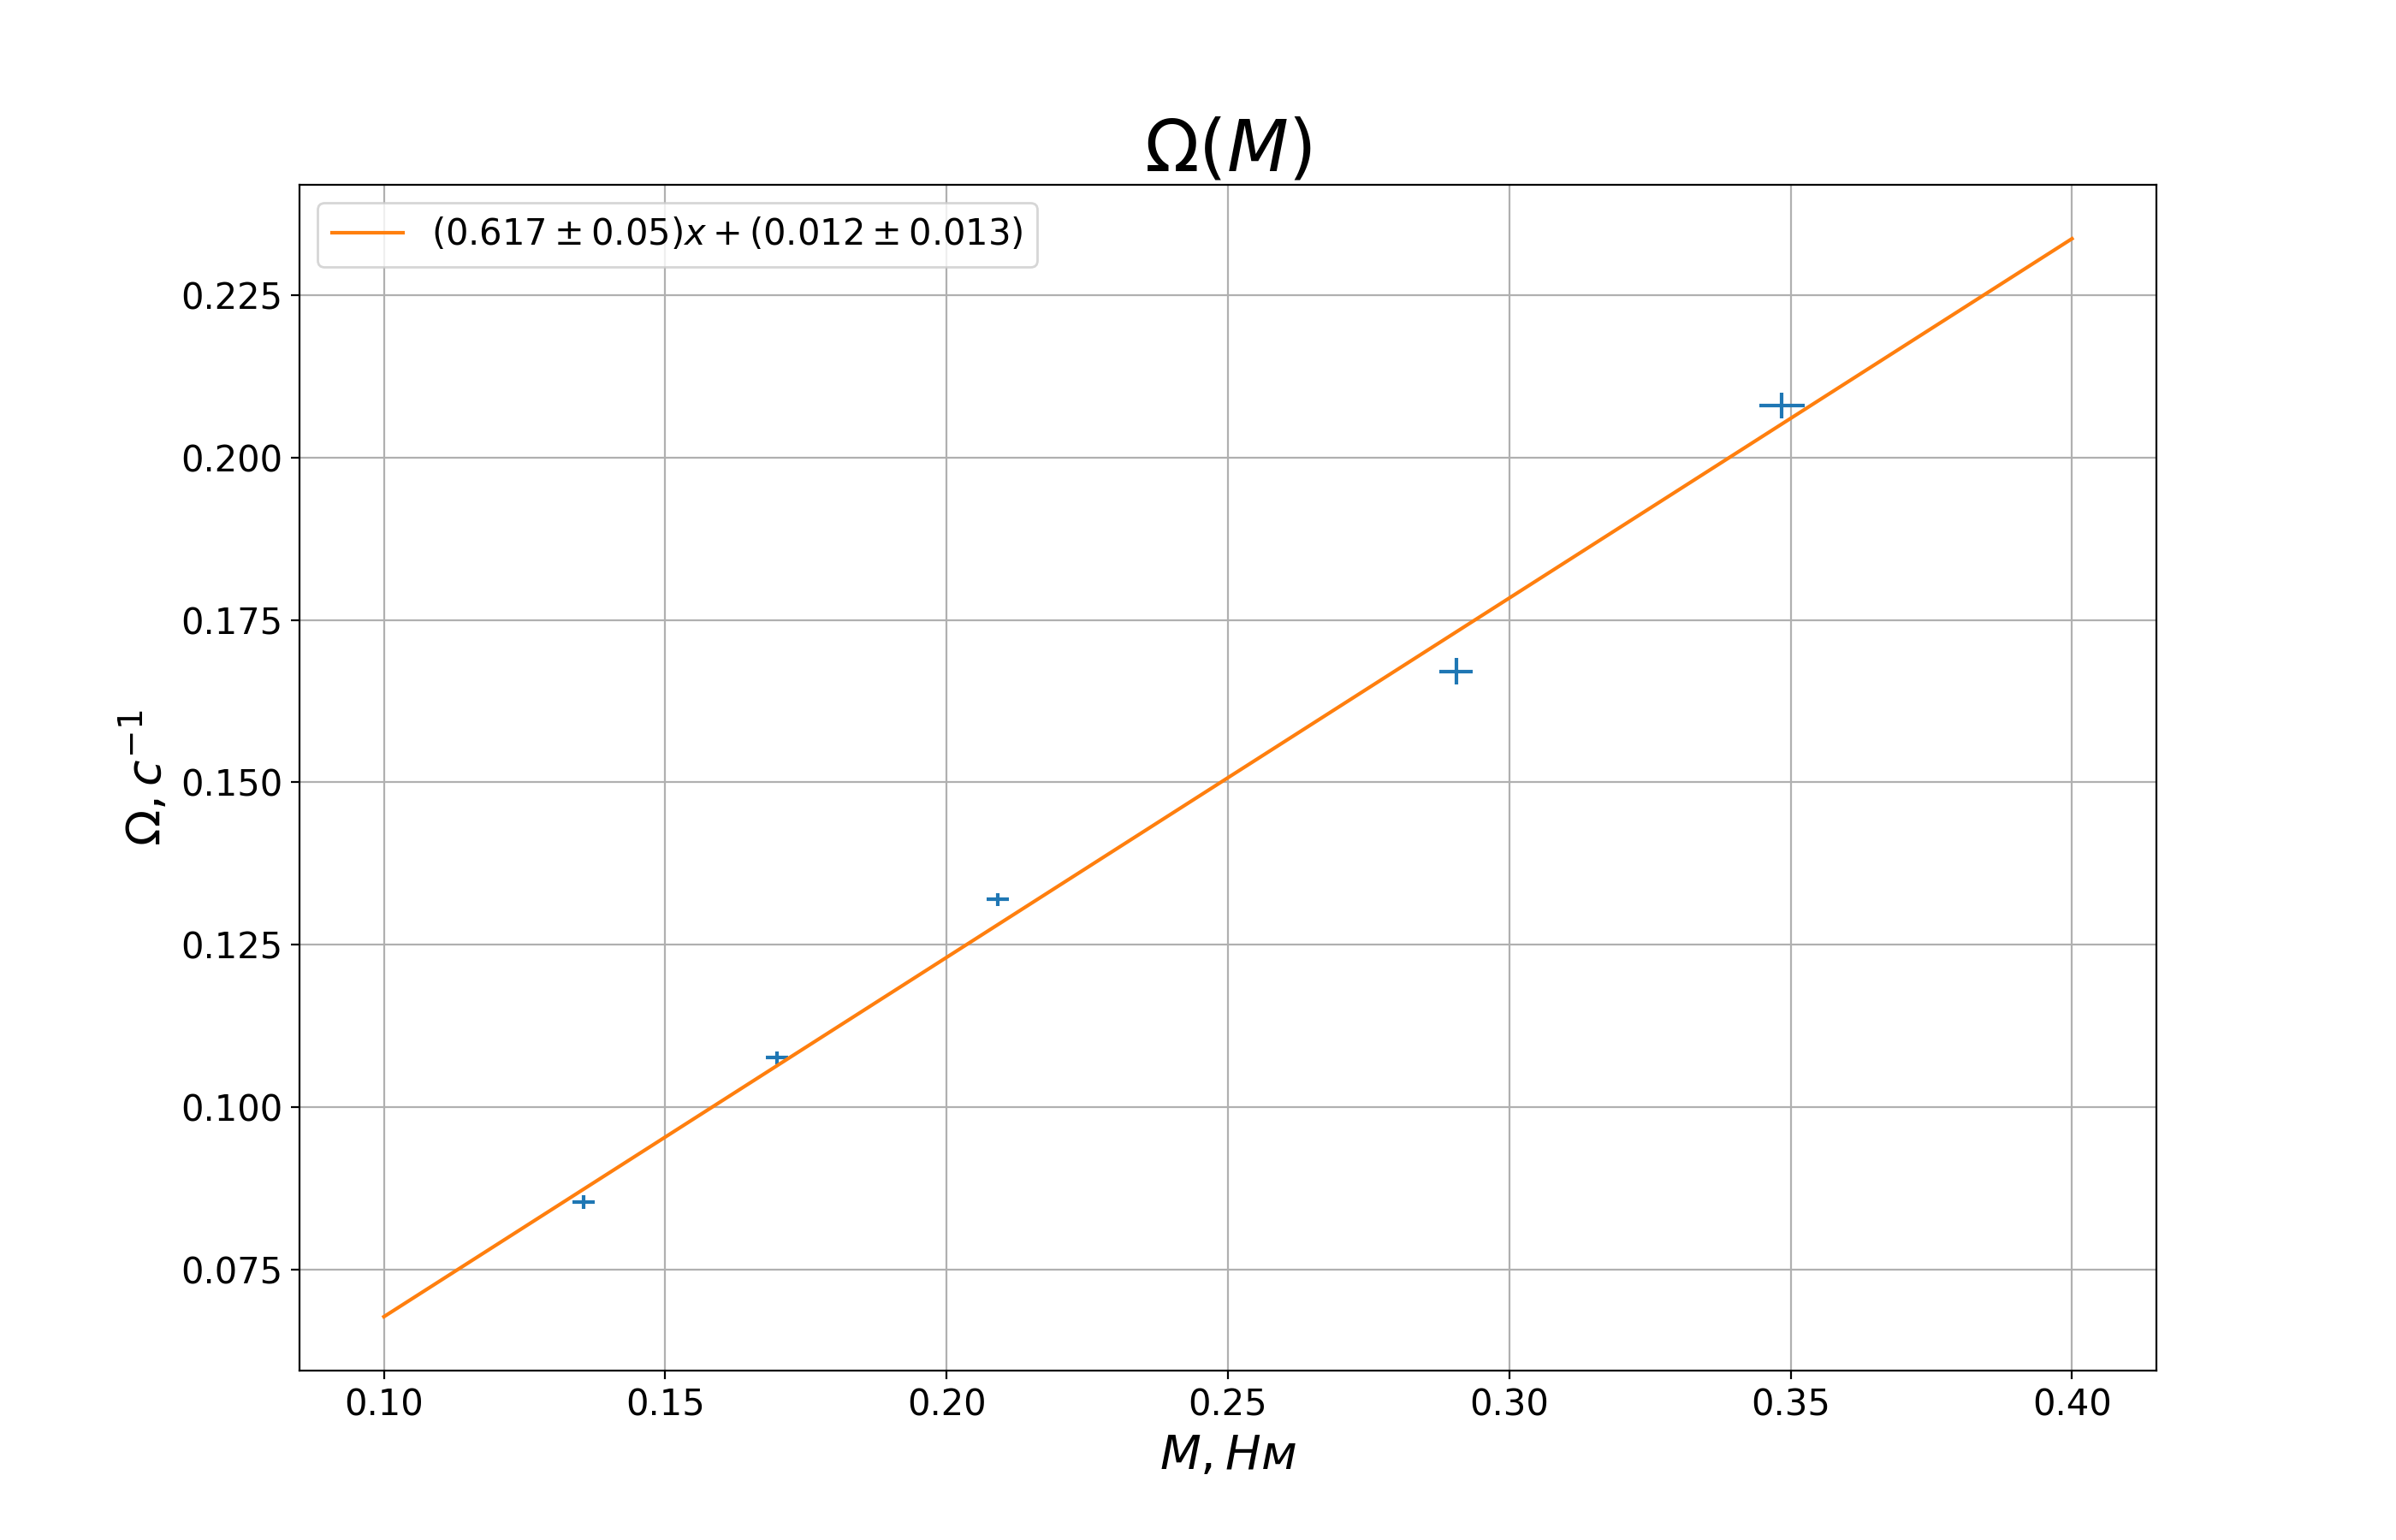
\includegraphics[width=1.20\textwidth]{plot.png}
        \caption{График $\Omega(M)$}
    \end{sidewaysfigure}
\end{document}

